\documentclass{article}
\usepackage{graphicx}
\usepackage{subfigure}
\usepackage{multirow}
\usepackage{wrapfig}
\usepackage{amssymb}
\usepackage{amsfonts, amsmath}
\usepackage{amsmath}
\usepackage{mathrsfs}
\usepackage{enumerate}
\usepackage[bookmarks=true]{hyperref}
\usepackage{amssymb,amsmath,amsthm,amsfonts}
\usepackage{mathrsfs}
\usepackage{dsfont}
\usepackage{enumerate}

%\newtheorem{mdef}{Definition}
%\newtheorem{theorem}{Theorem}
\newcommand{\eqsplit}[2]{
  \begin{equation}\label{#2}
    \begin{split}
      #1
    \end{split}
  \end{equation}}
\newcommand{\eqnsplit}[1]{
  \begin{eqnarray*}
    #1
  \end{eqnarray*}}
\newcommand{\tran}[1]{
  \tilde{#1}
}
\newcommand{\td}[2]{
  \frac{d #1}{d #2}
}
\newcommand{\pd}[2]{
  \frac{\partial #1}{\partial #2}
}
\newcommand{\ppd}[2]{
  \frac{\partial^2 #1}{\partial #2^2}
}
\newcommand{\pdd}[3]{
  \frac{\partial^2 #1}{\partial #2 \partial #3}
}
\newcommand{\otd}[1]{
  \frac{d}{d #1}
}
\newcommand{\opd}[1]{
  \frac{\partial}{\partial #1}
}
\newcommand{\oppd}[1]{
  \frac{\partial^2}{\partial #1^2}
}
\newcommand{\opdd}[2]{
  \frac{\partial^2}{\partial #1 \partial #2}
}
\newcommand{\ket}[1]{
  |#1\rangle
}
\newcommand{\bra}[1]{
  \langle#1|
}
\newcommand{\inn}[1]{
  \langle#1\rangle
}
\newcommand{\mean}[1]{
  \langle#1\rangle
}
\newcommand{\tr}{
  \text{tr}\,
}
\newcommand{\re}{
  \text{Re}\,
}
\newcommand\im{
  \text{Im}\,
}
\newcommand{\var}{
  \text{var}
}
\newcommand{\arcsinh}{
  \sinh^{-1}
}
\newcommand{\arccosh}{
  \cosh^{-1}
}
\newcommand{\erfc}{
  \text{erfc}
}
\newcommand{\E}{
  \mathbb{E}
}
\renewcommand{\P}{
  \mathbb{P}
}
\newcommand{\I}[1]{
  \mathbf{1}_{\{#1\}}
}
\newcommand{\1}[1]{
  \mathds{1}_{\{#1\}}
}
\newcommand{\diag}{
  \text{diag\,}
}
\newcommand{\M}{
  {\text{max}}
}
\newcommand{\m}{
  {\text{min}}
}
\newcommand{\ph}{
  {\text{arg}\,}
}
\newcommand\erf{
  \text{erf}
}
\renewcommand\vec[1]{
  \mathbf{#1}
}
\newcommand\mtx[1]{
  \mathbf{#1}
}
\newcommand\ed{
  \,{\buildrel d \over =}\,
}




\DeclareGraphicsExtensions{.pdf}
\begin{document}
How the maximum eigenvalue's distribution compares to Tracy-Widom:

\begin{figure}[htb!]
  \centering
  \includegraphics[scale=0.5]{../r/eigmax_TW_q0dot1.pdf}
  \caption{\small \it Comparison of the largest eigenvalue's
    distribution with Tracy-Widom. $q=N/T=0.1$}
  \label{fig:eig1_TW_q0.1}
\end{figure}

\begin{figure}[htb!]
  \centering
  \includegraphics[scale=0.5]{../r/eigmax_TW_q0dot2.pdf}
  \caption{\small \it Comparison of the largest eigenvalue's
    distribution with Tracy-Widom. $q=N/T=0.2$}
  \label{fig:eig1_TW_q0.2}
\end{figure}

Comparison between the empirical spectral density and the theoretical
density. The value of $v$ used to obtain the theoretical density is
the result of {\it maximum likelihood estimation}.
\begin{figure}[htb!]
  \centering
  \subfigure[q = 0.5, KL = 0.19]{
    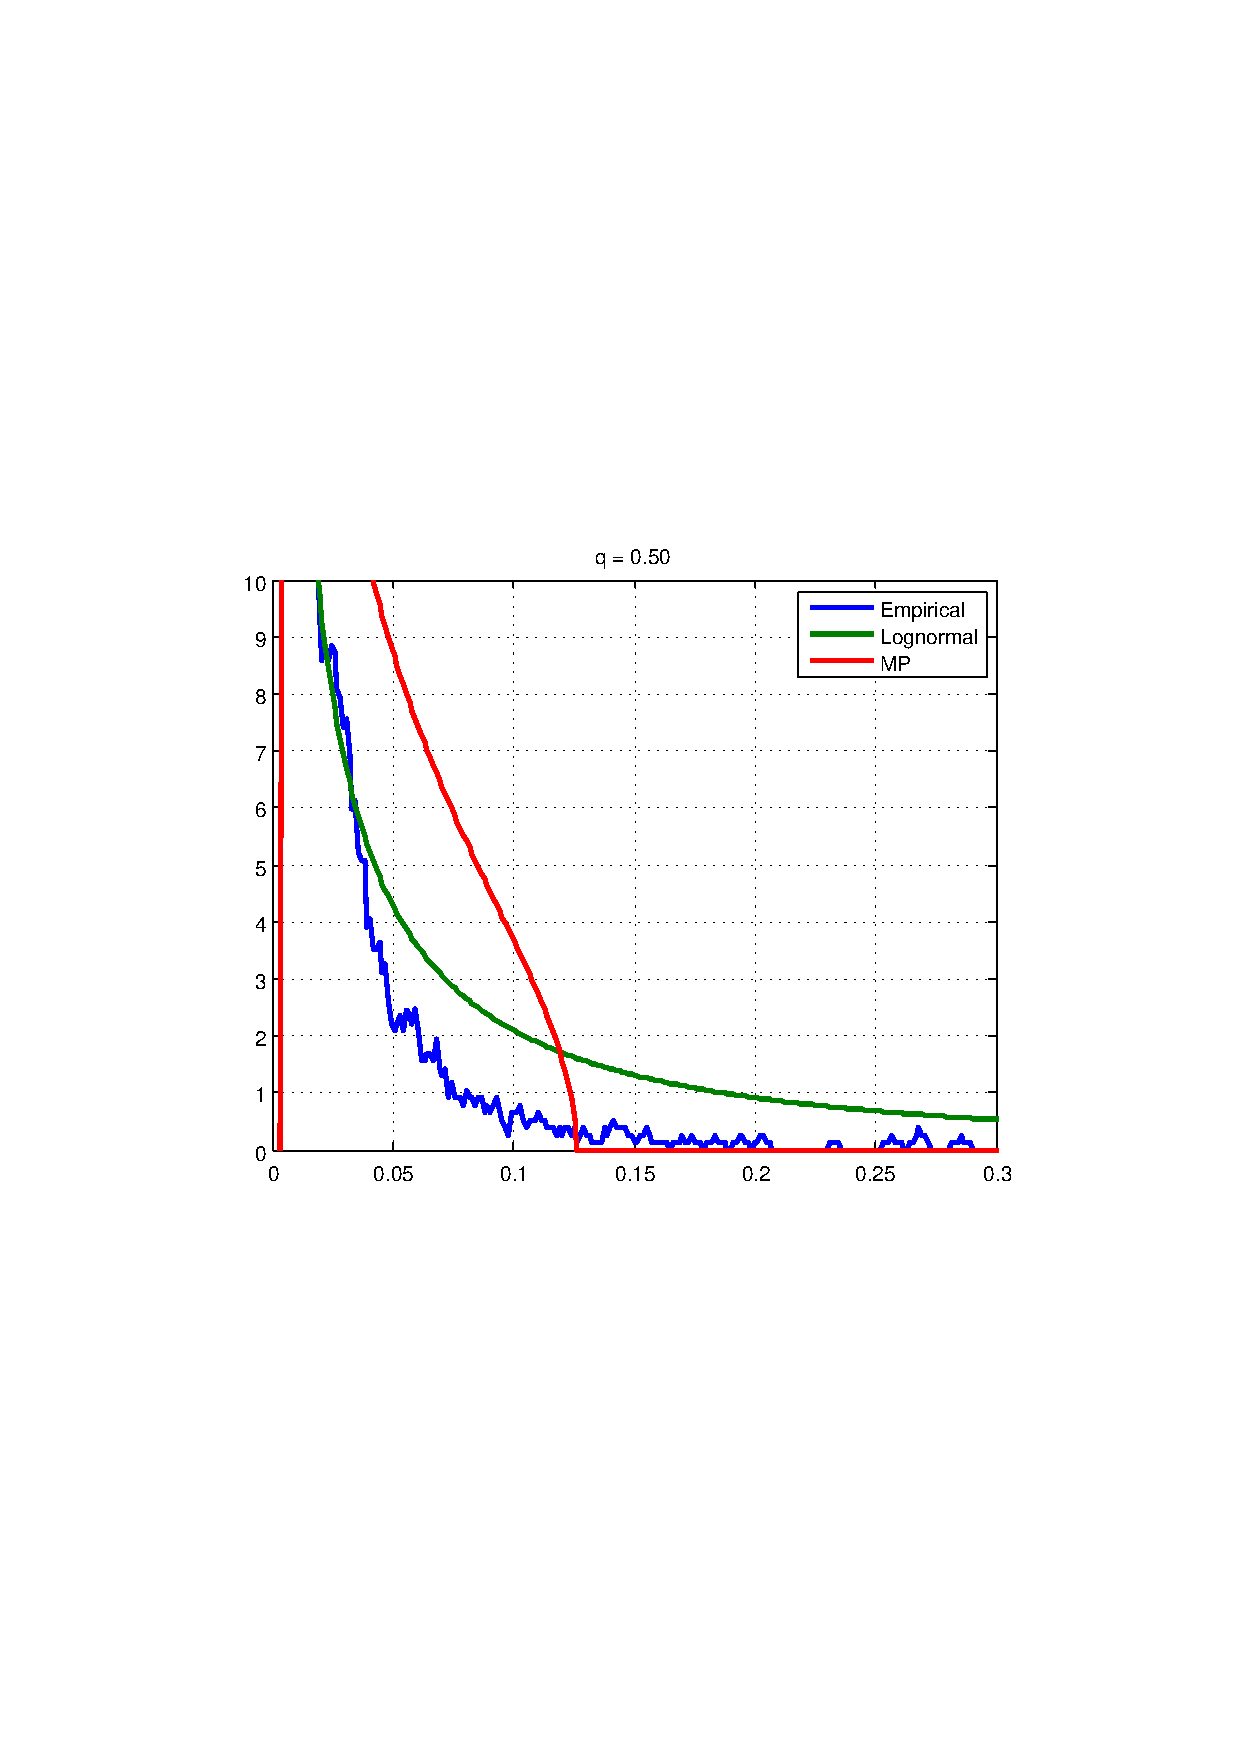
\includegraphics[scale=0.4, clip=true, trim=115 271 109
    204]{../pics/spectral_density_q0dot5.pdf}
  }
  \subfigure[q = 0.65, KL = 0.15]{
    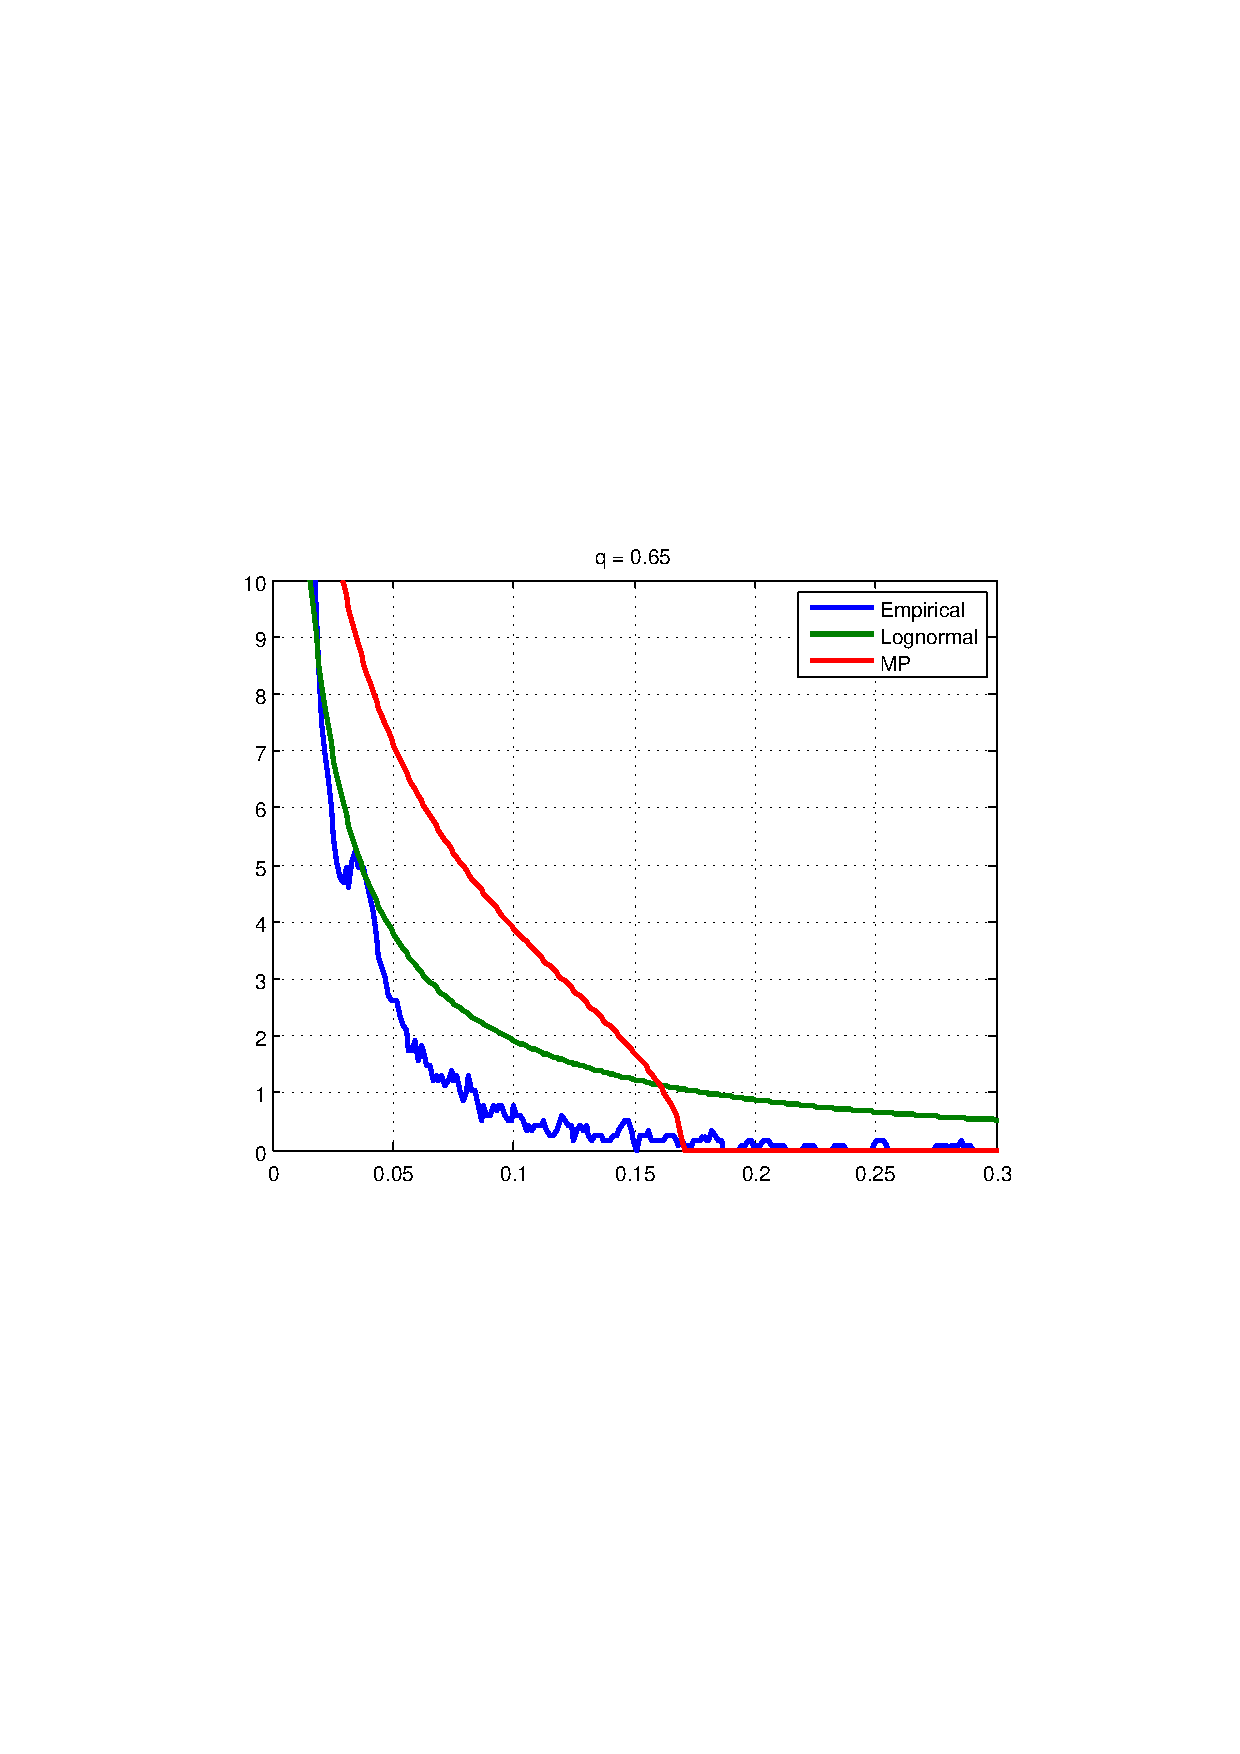
\includegraphics[scale=0.4, clip=true, trim=115 271 109
    204]{../pics/spectral_density_q0dot65.pdf}
  }
  \subfigure[q = 0.8, KL=0.14]{
    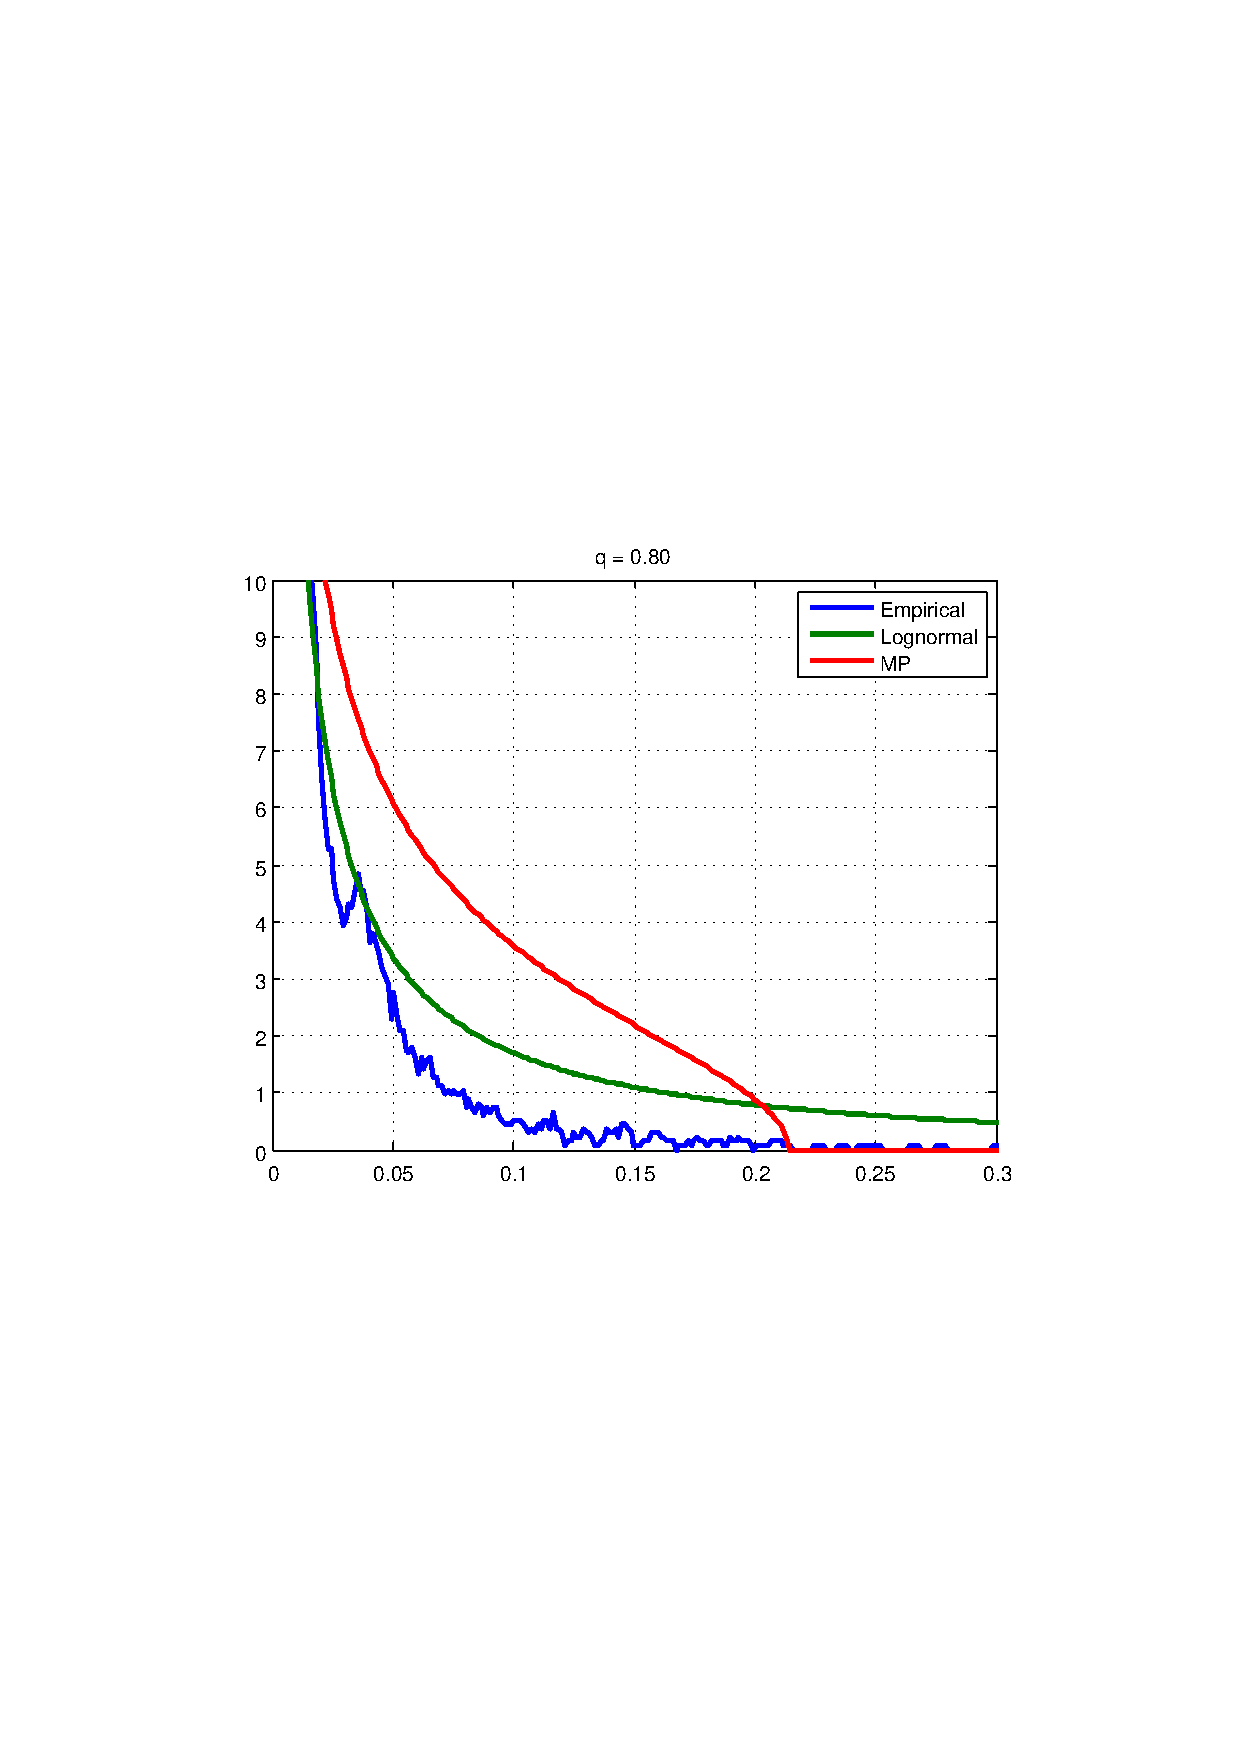
\includegraphics[scale=0.4, clip=true, trim=115 271 109
    204]{../pics/spectral_density_q0dot8.pdf}
  }
  \subfigure[q = 0.95, KL=0.15]{
    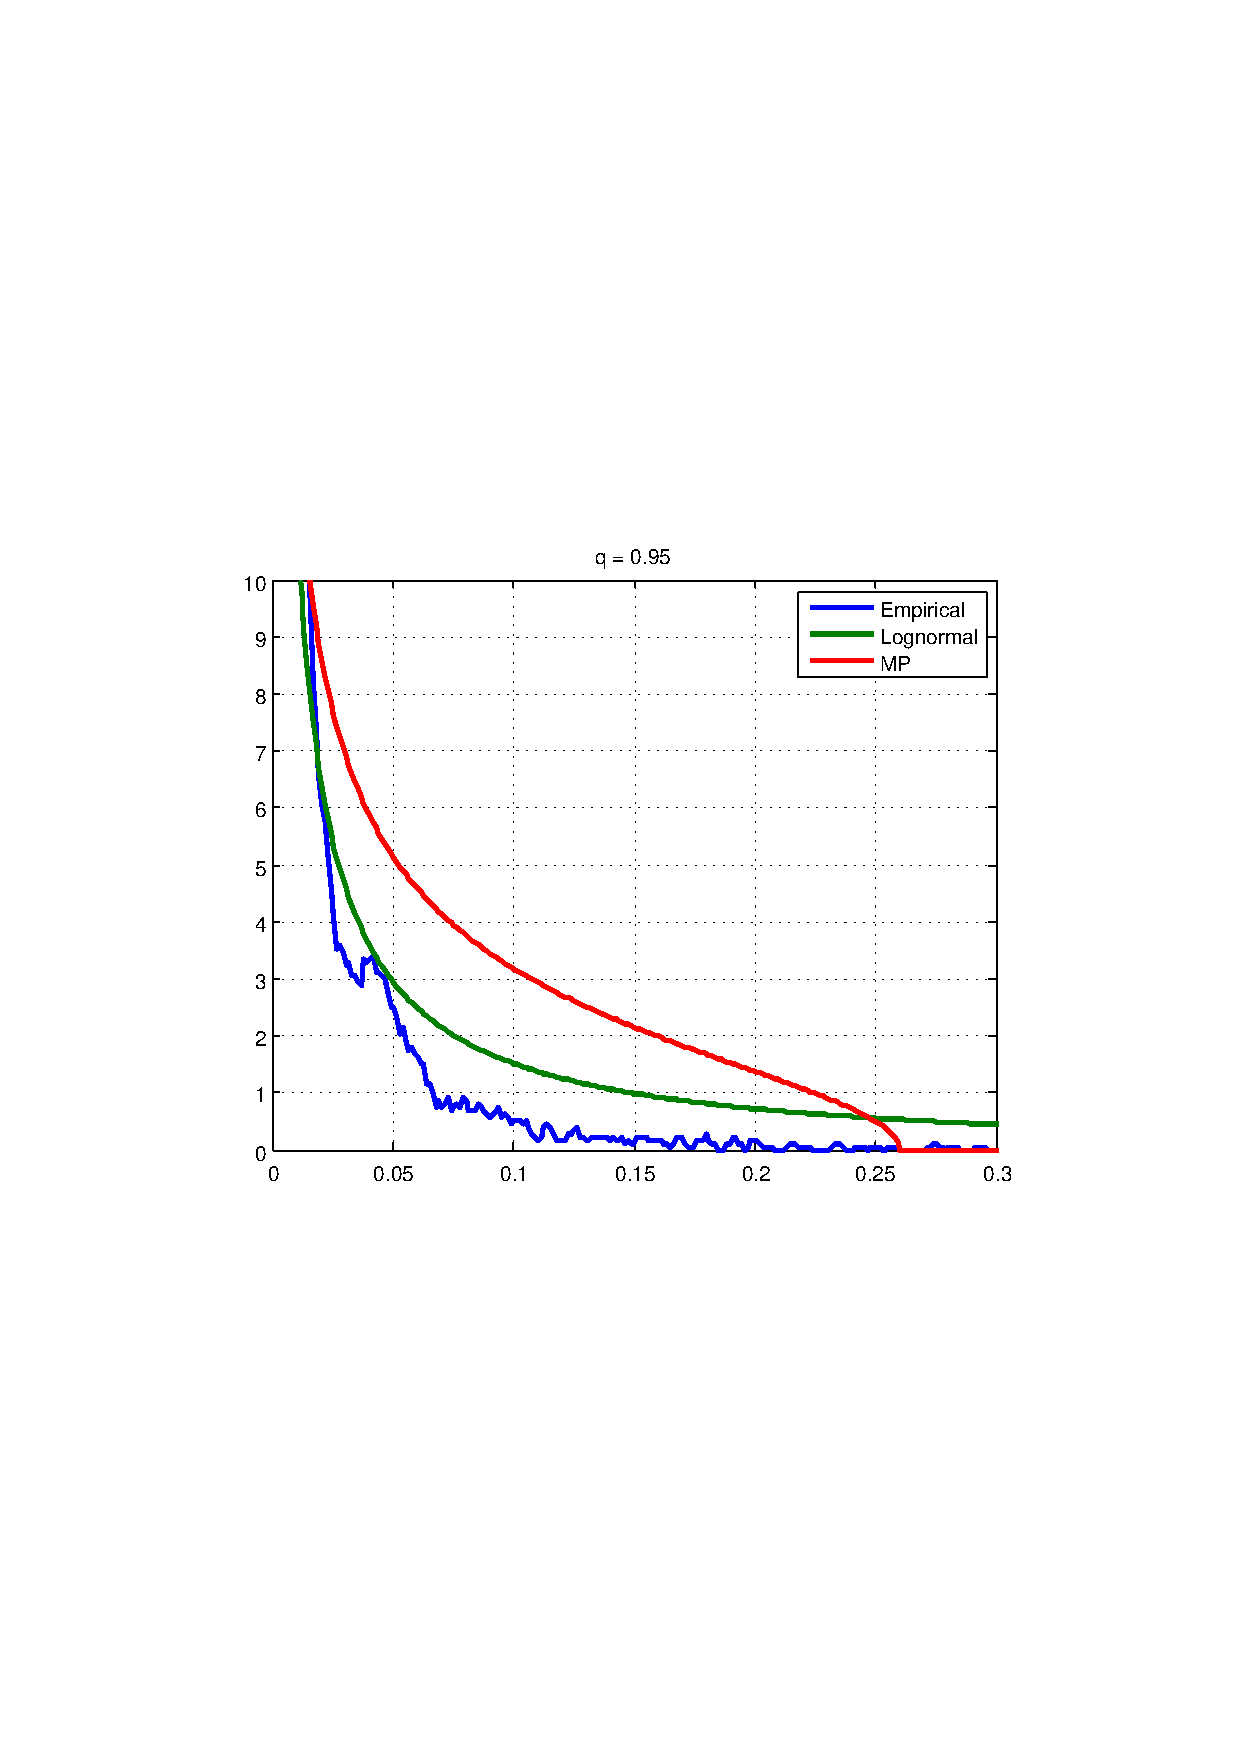
\includegraphics[scale=0.4, clip=true, trim=115 271 109
    204]{../pics/spectral_density_q0dot95.pdf}
  }
  \caption{\small \it Comparison of the empirical and theoretical
    spectral densities. The largest empirical eigenvalue ($\lambda_1$)
    is excluded. The rest is rescaled by $1/\lambda_1$. The
    theoretical density functions are ajusted accordingly. KL is the
    Kullback-Leibler divergence of the theoretical density function from
    the empirical density function. Only intervals on which the
    empirical density is non-zero are included in the calculation of
    KL.}
  \label{fig:spectral_density}
\end{figure}

\end{document}
